\pgfplotsset{compat=1.16}
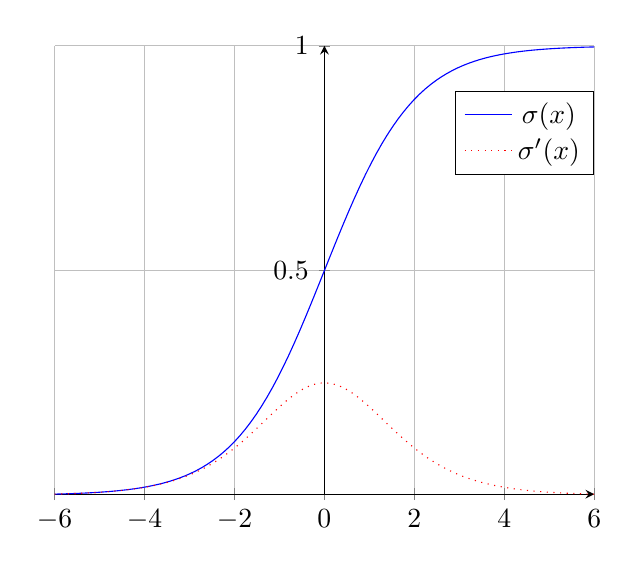
\begin{tikzpicture}[declare function={sigma(\x)=1/(1+exp(-\x));
sigmap(\x)=sigma(\x)*(1-sigma(\x));}]
\begin{axis}%
[
    grid=major,     
    xmin=-6,
    xmax=6,
    axis x line=bottom,
    ytick={0,.5,1},
    ymax=1,
    axis y line=middle,
    samples=100,
    domain=-6:6,
    legend style={at={(1,0.9)}}     
]
    \addplot[blue,mark=none]   (x,{sigma(x)});
    \addplot[red,dotted,mark=none]   (x,{sigmap(x)});
    \legend{$\sigma(x)$,$\sigma'(x)$}
\end{axis}
\end{tikzpicture}